\section{DC motoren}
Dette appendix beskæftiger sig med bestemmelsen af motorparametrene.
\subsection{DC Motor karakteristik}
DC Motoren kan modelleres efter diagrammet på fig. \todo[inline]{kredsløbsdiagram skal indsættes}\todo[inline]{Kildehenvisning til DC motor model}.
Ligningen for $V_m$ er givet ved ligning \ref{eq:Vm_transient0}.
\begin{equation}
	V_m(t)=L_m \cdot \frac{\mathrm d}{\mathrm d t} \big( i_m(t) \big)+R_m \cdot i_m(t) + V_{EMF}(t)
	\label{eq:Vm_transient0} 
 \end{equation}
Den modelektromotoriske kraft, $V_{EMF}$ er givet ved ligning \ref{eq:VEMF}.
\begin{equation}
	V_{EMF}(t) = K_b \cdot \omega(t)
	\label{eq:VEMF}
\end{equation}
Med ligning \ref{eq:VEMF} kan ligning \ref{eq:Vm_transient0} omskrives til ligning \ref{eq:Vm_transient1}.
\begin{equation}
	V_m(t)=L_m \cdot \frac{\mathrm d}{\mathrm d t} \big( i_m(t) \big)+R_m \cdot i_m(t) +K_b \cdot \omega(t)
	\label{eq:Vm_transient1} 
 \end{equation}

\subsection{Eksperiment 1}
\label{ss:eksperiment1}
\subsubsection{Formål}
Bestemmelse af motorens ækvivalente resistans, $R_m$.
\subsubsection{Teori}
Forhindres motoren i at rotere, vil vinkelhastigheden være nul.
Hvis man påfører motoren en DC-spænding $V_m$,
og venter til motorens respons har nået steady-state,
så vil strømmen igennem motoren være konstant.
Her vil ligning \ref{eq:Vm_transient1} kunne omskrives til ligning \ref{eq:resistans_E1}.
\begin{equation}
	V_m=R_m \cdot i_m
	\label{eq:resistans_E1} 
 \end{equation}
Målinger af sammenhørende steady-state værdier for strøm $i_m$ og spænding $V_m$
kan altså bruges til bestemmelse af den ækvivalente resistans $R_m$.
\subsubsection{Fremgangsmåde}
Motoren låses fast vha. en skiftenøgle og påføres en lav spænding.
Efter nogle sekunder, når transientresponsen er væk,
måles spændingen over og strømmen igennem motoren med multimetre.
Værdierne noteres, og forsøget gentages ved andre spændinger.
De anvendte multimetre er af typen TTi 1604.
\subsubsection{Måleresultater}
I tabel \ref{tb:resistans} findes målingerne af strøm og spænding.
\begin{figure}[th!]
	\centering
	%\begin{tabular}{r|r}
%$V_m$ [V]&$i_m$ [A]\\\hline
%0,509&0,094 \\ %0,5093&0,094 \\
%0,883&0,172 \\ %0,8833&0,172
%1,481&0,297 \\ %1,4809&0,297 
%1,940&0,391 \\ %1,9404&0,391
%2,345&0,470 \\ %2,3448&0,470
%2,788&0,555 \\ %2,7879&0,555
%3,182&0,638 \\ %3,1823&0,638
%3,465&0,664 \\ %3,4652&0,664
%3,835&0,746 \\ %3,8346&0,746
%4,067&0,765 \\ % 4,067&0,765
%4,292&0,830 \\ %4,292&0,830 
%\end{tabular}


\begin{tabular}{r|r|r|r|r|r|r|r|r|r|r|r}
$V_m$ [V]&0,509&0,883&1,1481&1,940&2,345&2,788&3,182&3,465&3,835& 4,067&4,292\\\hline
$i_m$ [A]&0,094&0,172&0,297 &0,391&0,470&0,555&0,638&0,664&0,746&0,765&0,830
\end{tabular}
	\captionsetup{type=table}
	\caption[Sammenhørende værdier af DC spænding og strøm]
			{Sammenhørende værdier af DC spænding over og strøm gennem rotationslåst motor.}
	\label{tb:resistans}
\end{figure}
\subsubsection{Databehandling}
Den målte strøm-spændingskarakteristik for DC-motoren er indtegnet på figur \ref{fig:resistans0}.
\begin{figure}[th!]
	\centering
	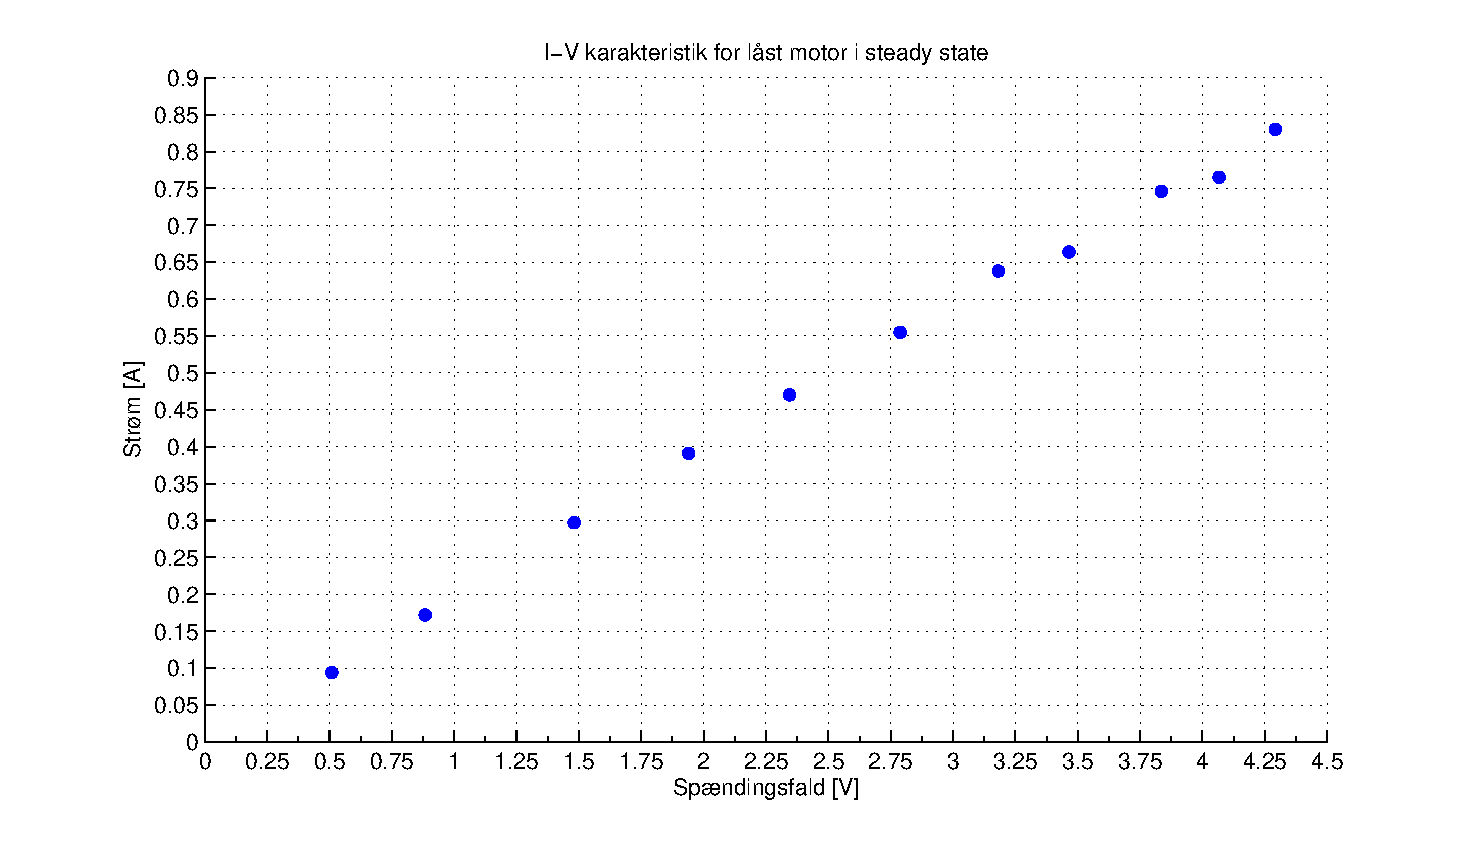
\includegraphics[width=1\textwidth]{./graphics/resistans1.eps}
	\caption[Strøm-spændingskarakteristik for rotationslåst DC-motor]{Strøm-spændingskarakteristik for rotationslåst DC-motor ved steady-state.}
	\label{fig:resistans0}
\end{figure}
Som det ses på figur \ref{fig:resistans0} er sammenhængen mellem strøm og spænding
tilnærmelsesvis lineær, og en lineær regression på dataene vil altså give en tilnærmet værdi for $R_m$.
$R_m$ er ved lineær regression beregnet til 5,21 $\Omega$.\todo{Flere decimaler?}

Den i forsøget mindste afsatte effekt i motoren er 48 mW.
\subsubsection{Diskussion}
Da sammenhængen mellem strøm og spænding i målingerne er tilnærmelsesvis lineær,
vurderes den fundne værdi for $R_m$ at være meget nøjagtig,
om ikke andet, så for effektafsættelser i motoren på mindst 48 mW.
\subsubsection{Konklusion}
Motorens ækvivalente resistans, $R_m$ er vha. sammenhørende målinger af strøm og spænding
for en rotationslåst motor, ved effektafsættelser på 48 mW og højere,
blevet bestemt til 5,21 $\Omega$.\todo{Flere decimaler?}
\subsection{Eksperiment 2}
\subsubsection{Formål}
Bestemmelse af motorens ækvivalente induktans, $L_m$.
Der er benyttet to forskellige metoder til bestemmelsen af induktansen.
Metode 1 tager udgangspunkt i tidskonstanten for et RL-kredsløb,
mens metode 2 tager udgangspunkt i faseforskellen mellem forskellige komplekse impedanser i serie.
\subsubsection{Teori}
\paragraph{Metode 1}
Forhindres motoren i at rotere, vil vinkelhastigheden som beskrevet i afsnit \ref{ss:eksperiment1} være nul.
Ved denne metode er vi interesseret i systemets transientrespons, hvor strømmen $i_m$ ikke er konstant.
Forbindes en modstand $R_s$ i serie med DC-motoren som vist på fig. %\ref{fig:e2_rl1}
\todo[inline]{Indsæt kredsløbsdiagram med Rs}
vil der være tale om et RL-kredsløb, med en tidskonstant $\tau$ givet ved ligning \ref{eq:rltimeconstant}.
Transientresponsen for alle strømme og spændingsfald i kredsløbet har denne tidskonstant.
\todo[inline]{Indsæt kilde eller forklaring til RL-tidskonstant.}
\begin{equation}
	\tau=\frac{L_m}{R_m+R_s}
	\label{eq:rltimeconstant} 
 \end{equation}
Tidskonstanten er et mål for tiden det tager systemet at opnå ca. 63,2 \% af slutværdien.\todo{D\&B-kilde}
For en (eksponentielt) aftagende kurve med tidskonstanten $\tau$ kan tidskonstanten aflæses som
tidsforskellen mellem to niveauer V0 og V1, hvor V1 er ca. 36,8 \% af V0.

Ved omskrivning af ligning \ref{eq:rltimeconstant} kan induktansen altså bestemmes vha. ligning \ref{eq:induktans0}.
\begin{equation}
	L_m=\tau\cdot\left(R_m+R_s\right)
	\label{eq:induktans0} 
 \end{equation}
\paragraph{Metode 2}
Forhindres motoren i at rotere, vil vinkelhastigheden som beskrevet i afsnit \ref{ss:eksperiment1} være nul.
Ved denne metode er vi interesseret i systemets steady-state respons.
Forbindes en modstand $R_{s1}$ i serie med DC-motoren som vist på fig. %ref{fig:e2_rl2}
\todo[inline]{Indsæt kredsløbsdiagram med Rs1 og AC-forsyning med DC offset}
vil impedansen $\mathbf{Z_m}$ af DC-motoren være givet ved ligning \ref{eq:zm_0}.
\begin{equation}
	\mathbf{Z_m}=R_{s1}\cdot\frac{\mathbf{V_1}-\mathbf{V_2}}{\mathbf{V_2}}
			=R_{s1}\cdot\left(\frac{\mathbf{V_1}}{\mathbf{V_2}}-1\right)
			=R_{s1}\cdot\left(\frac{A_1}{A_2}\cdot{e}^{\phi}-1\right)
	\label{eq:zm_0} 
 \end{equation}
Bemærk at spændingsfaldene noteres med fed skrift for at indikere at her er tale om phasors (komplekse tal),
at $A_1$ og $A_2$ angiver amplituderne af $\mathbf{V_1}$ og $\mathbf{V_2}$,
samt at $\phi=\phi_1-\phi_2$ angiver faseforskellen mellem de to signaler.
Denne faseforskel kan også udtrykkes ved tidsforsinkelsen $\Delta{t}$ ganget med vinkelfrekvensen $\omega$.
Ligning \ref{eq:zm_1} angiver impedansen på rektangulær form.
\begin{equation}
	\mathbf{Z_m}=R_{s1}\cdot\left(\frac{A_1}{A_2}\cdot{\cos (\phi)}-1\right)	%Realdel
	+\mathbf{j}\cdot{R_{s1}}\cdot\frac{A_1}{A_2}\cdot\sin(\phi)	%Imaginærdel
	\label{eq:zm_1} 
 \end{equation}
Samtidig vides det, at den rotationslåse motors impedans består af resistansen $R_m$ samt
reaktansen $X_m$, hvor $X_m$ er reaktansen for en spole, altså $\omega\cdot{L_m}$.
Motorens impedans kan altså også beskrives ved ligning \ref{eq:zm_2}, hvor $\mathbf{j}$ er den imaginære enhed.
\begin{equation}
	\mathbf{Z_m}=R_m+\mathbf{j}\cdot\omega\cdot{L_m}
	\label{eq:zm_2} 
 \end{equation}
Sættes ligningerne \ref{eq:zm_1} og \ref{eq:zm_2} lig med hinanden
kan man altså udtrykke resistansen $R_m$ og induktansen $L_m$ som funktioner
af faseforskellen på $\mathbf{V_1}$ og $\mathbf{V_2}$,
hvilket giver ligningerne \ref{eq:Rm_0} og \ref{eq:Lm_0}.
\begin{equation}
	\mathbf{R_m}=R_{s1}\cdot\left(\frac{A_1}{A_2}\cdot{\cos (\phi)}-1\right)
	\label{eq:Rm_0} 
 \end{equation}
\begin{equation}
	\mathbf{L_m}=R_{s1}\cdot\frac{A_1}{A_2}\cdot\sin(\phi)
	\label{eq:Lm_0} 
 \end{equation}
\subsubsection{Fremgangsmåde}
\paragraph{Metode 1}
En modstand $R_s$ måles efter med et multimeter og fobindes i serie med DC-motoren
som på figur %\ref{fig:e2_rl1}
.
Kredsløbet bestående af DC-motoren og $R_s$ påføres en kendt spænding.
Strømmen gennem kredsløbet afbrydes på strømforsyningen og spændingsfaldet
over $R_s$ måles med et oscilloskop.
Dataene eksporteres og tidskonstanten bestemmes herudfra.
Forsøget gentages.

Det anvendte multimeter er af typen TTi 1604,
og oscilloskopet er af typen \todo{Oscilloskop?}.

\paragraph{Metode 2}
\subsubsection{Måleresultater}
\paragraph{Metode 1}
Seriemodstanden $R_s$ er blevet målt til 61,77 $\Omega$.
På figur \ref{fig:induktans0} er transientresponsen for spændingsfaldet over $R_s$ indtegnet
sammen med de to spændingsniveauer, hvorudfra tidskonstanten bestemmes.
\begin{figure}[th!]
	\centering
	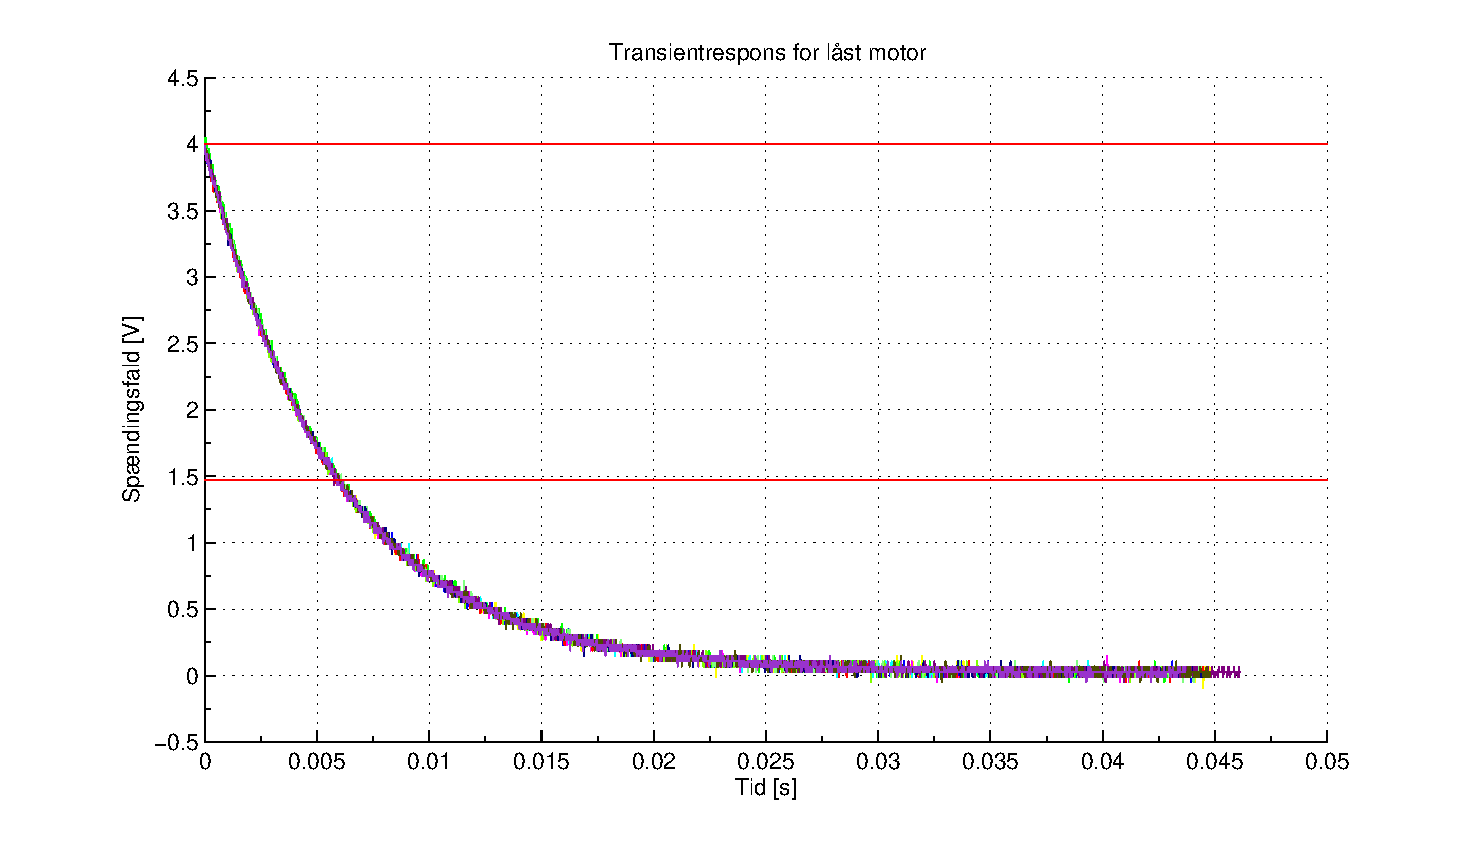
\includegraphics[width=1\textwidth]{./graphics/induktans0.eps}
	\caption[Transientrespons for låst motor]
		{Transientrespons for låst motor. De to vandrette røde linjer angiver spændingsniveauerne til bestemmelse af tidskonstanten.
		Den øverste linje er ved 4 V, mens den nederste linje er ved 4 V $\cdot \frac{1}{e}$.}
	\label{fig:induktans0}
\end{figure}
Figur \ref{fig:induktans0} viser flere målingers transientrespons.
\paragraph{Metode 2}
\subsubsection{Databehandling}
\paragraph{Metode 1}
For hver måling af transientresponsen, vist i figur \ref{fig:induktans0} er induktansen blevet
bestemt ved brug af ligning \ref{eq:induktans0}.
Gennemsnitsinduktansen er ved denne metode blevet fundet til $L_m=0.395$ H.
\paragraph{Metode 2}
\subsubsection{Diskussion}
\subsubsection{Konklusion}


\subsection{Eksperiment 3}
\subsubsection{Fremgangsmåde og forsøgsopstilling}
\subsubsection{Databehandling}
\subsubsection{Konklusion}


\subsection{Eksperiment 4}
\subsubsection{Fremgangsmåde og forsøgsopstilling}
\subsubsection{Databehandling}

\subsubsection{Konklusion}

\subsection{Opsummering af DC motorparameter}